% $Id:evaluation.tex  $
% !TEX root = main.tex

\chapter{Evaluation}
\label{cha:experiments}
\section{Setup}
The experiments were run using the Gazebo ros simulator and Carla simulator on a computer with the following specifications:
\begin{itemize}
    \item CPU: AMD Ryzen 9 8945HS 
    \item RAM: 16GB
    \item GPU: NVIDIA GeForce GTX 4060 Ti
    \item OS: Ubuntu 20.04 LTS 
    \item Ros Version: Noetic
    \item Python Version: 3.9
\end{itemize}
As a machine learning framework, Tensorflow 2.18\footnote{Tensorflow: \url{https://www.tensorflow.org}} was used.

\subsection{Carla}
Many options were taken in count while selecting environment to apply the transfer learning technique. The first one was CARLA \cite{CARLA}, which provides a realistic and dynamic context for autonomous driving research. In the frame of the MDP a reward signal was chosen to incentivize the agent to maintain a target speed of 50 km/h. The simulation environment for this study is the CARLA urban driving simulator.

Given that this thesis is employing a Twin Delayed Deep Deterministic Policy Gradient for decision-making, the action space has three continuous signals that can be powered: steering the vehicle, Throttle the vehicle, or break, CARLA simulator provides a way to manually shift gears and press the hand break, however in this experiment the car is only going to be able to move forward and the the gear shifting is going to be automatic. The vehicle is going to have one sensor only which is going to be an rgb frontal camera attached to the roof of the vehicle which is going to produce images of 3 rgb channels of 480 x 640 pixels. The reward function is designed to encourage the agent to reach and sustain the desired speed of $50km/h$ while navigating through the environment. This approach ensures that the agent learns to balance the need for speed with the challenges of urban driving, such as handling turns and avoiding obstacles. To achieve this, the agent receives a penalty of $-1$ for every step taken that is not above the $50km/h$, and gets a penalty of $-200$ for a collision and a negative reward of $-15$ every time it changes lane in a forbidden area.

\begin{figure}[!ht]
    \centering

    \subfloat[][Carla catalogue Townt 5 Overview.]{
        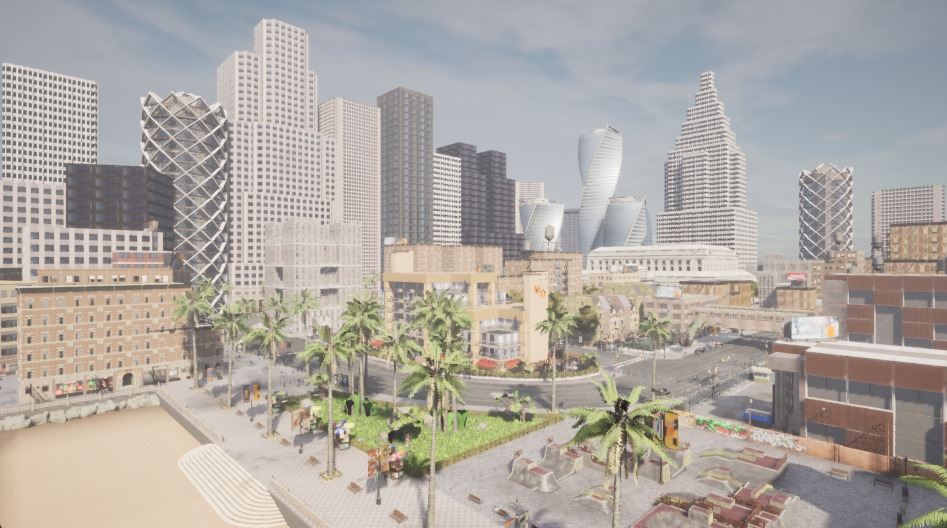
\includegraphics[width=0.6\textwidth]{figures/town5_carla_view1.png}
    }

    \subfloat[][Carla catalogue Townt 5 Overview.]{
        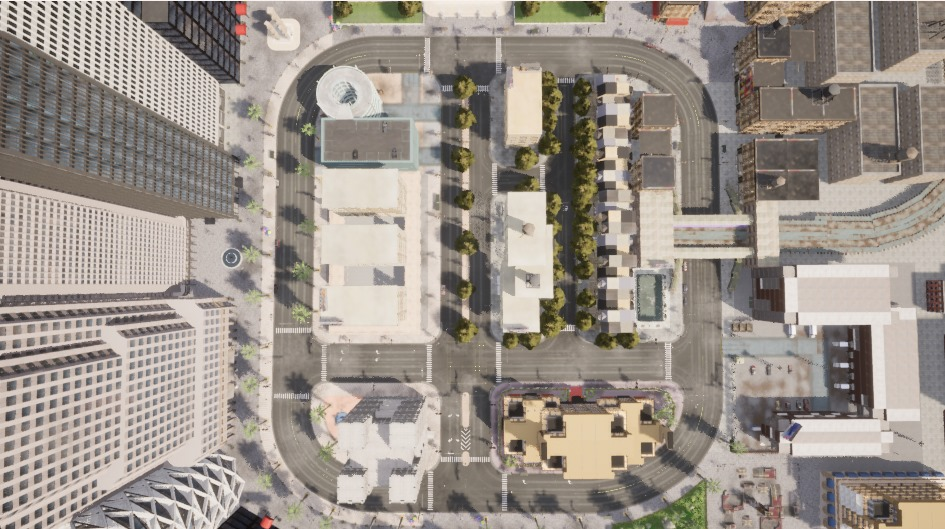
\includegraphics[width=0.6\textwidth]{figures/town5_carla_top_view.png}
    }

    \caption{Town 5 of Carla catalogue.}
    \label{fig:town 5 carla}
\end{figure}

\cite[Xception]{XCeption} is a 71 layer deep convolutional neural network which has over 23 millions trainable parameters. It was utilized to act as a policy function of the DDPG algorithm, for the critic network, a 4 layered of convolutional model followed by 2 dense layers was used to predict the value function of the actor in the environment.

The agent in the simulator was chosen to be a Cybertruck, model provided by the simulator as shown in figure \ref{cybwertruck carla}. CARLA provides in its catalogue a list of maps for use. For the experiment it was used the \ref{fig:town 5 carla} is an urban area nestled against conifer-covered hills, featuring a raised highway and expansive multilane roads with several major intersections.

\begin{figure}[ht]
    \centering
    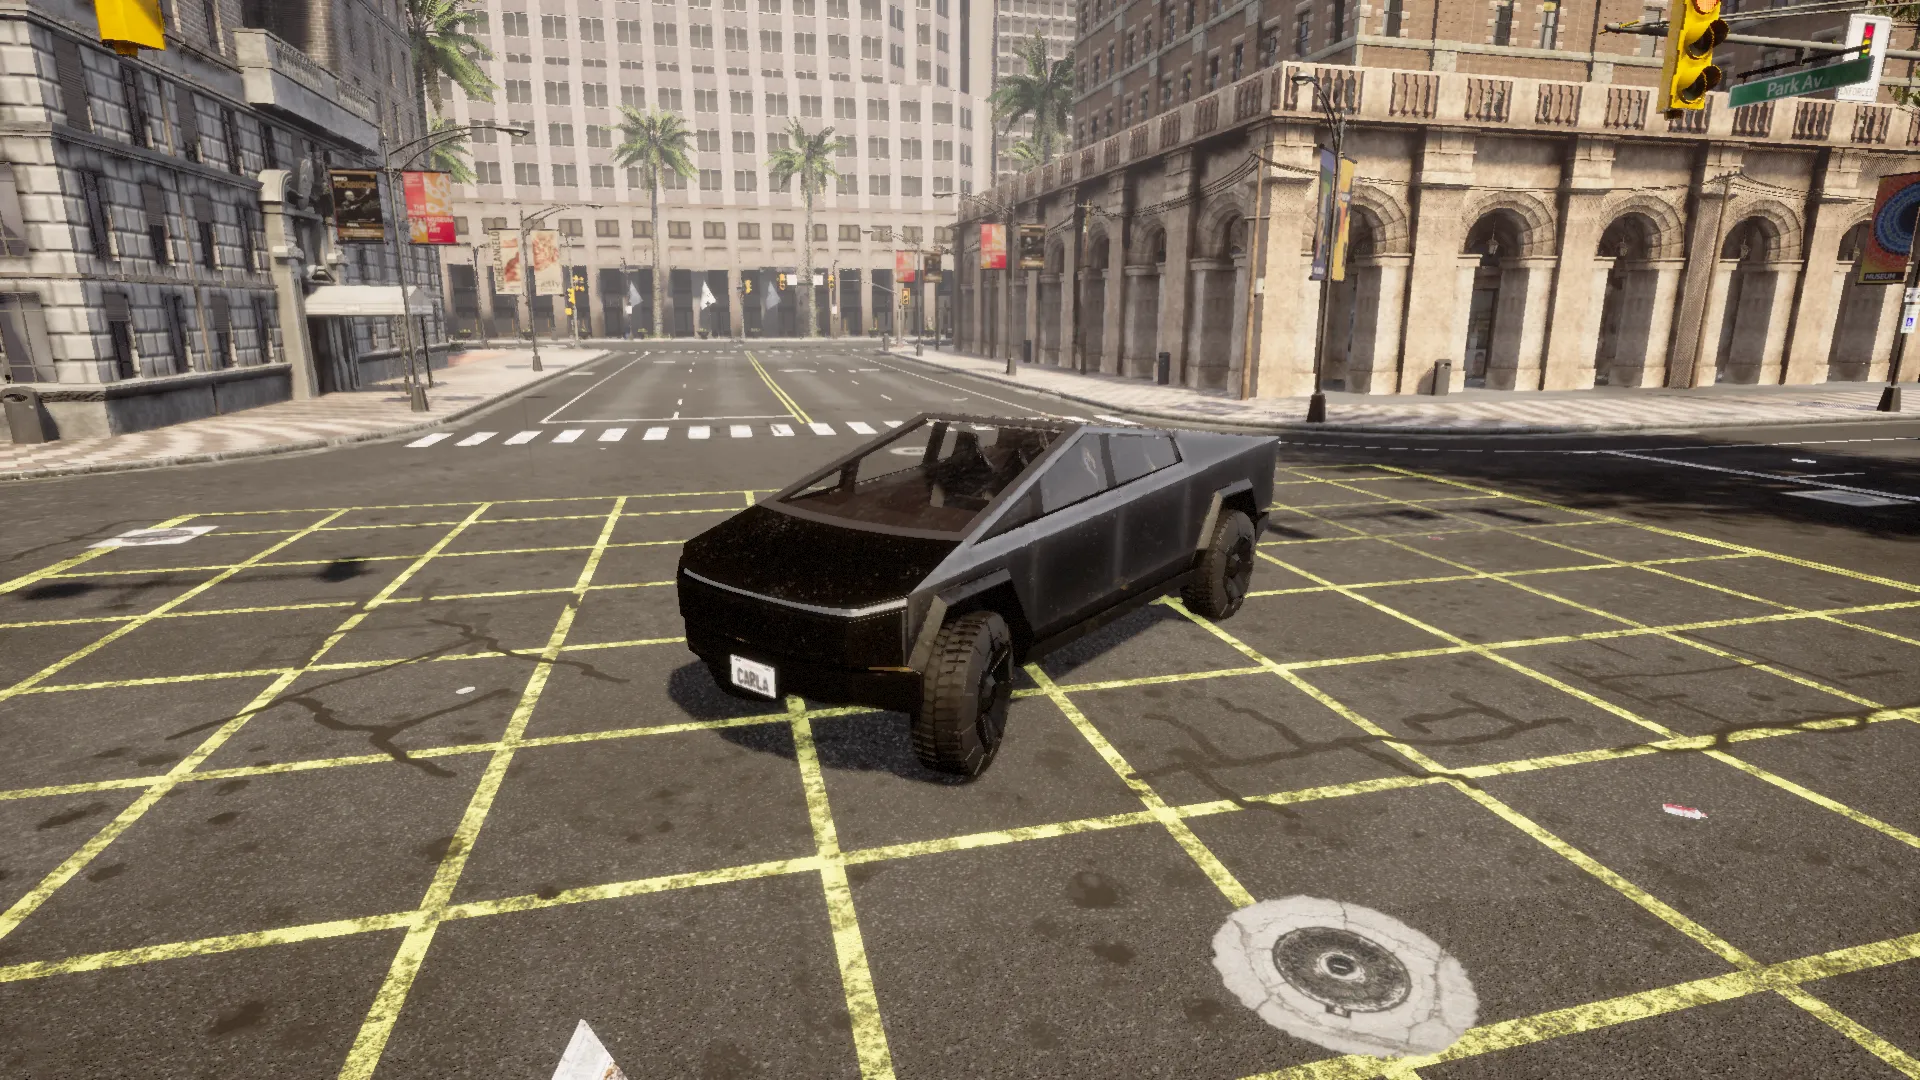
\includegraphics[width=0.8\textwidth]{./figures/tesla_cybertruck_carla.png}
    \caption{Cybertruck model in Carla environment in Town 5.}
    \label{cybwertruck carla}
\end{figure}

\subsection{Gazebo ROS}
The next environment was developed in Gazebo simulator and the Turtlebot3 mobile base shown in figure \ref{fig: tb3 model burger}, a differential mobile base with a Lidar\footnote{Laser Distance Sensor: https://emanual.robotis.com/docs/en/platform/turtlebot3/appendix\_lds\_01/} to sense the environment on a range of 24 degrees around the mobile base. The Turtlebot3 is a versatile and widely used platform in robotics research and education, making it suitable for various applications, including autonomous navigation and mapping\footnote{Turtlebot3: \url{https://emanual.robotis.com/docs/en/platform/turtlebot3/overview/}}.

As mentioned in algorithm \ref{al: td3}, two architecture of neural networks has to be constructed, one to perform as a critic and the other one as an actor/policy.

\begin{figure}[ht]
    \centering
    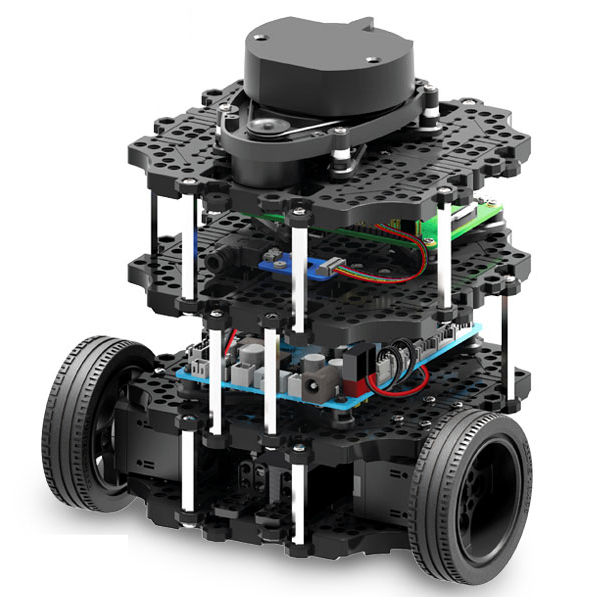
\includegraphics[width=0.2\textwidth]{./figures/turtlebor3_burger.png}
    \caption{Turtlebot3 model Burger.}
    \label{fig: tb3 model burger}
\end{figure}

The neural network begins with two input layers composed of 28 and 1 units, serving as the entry point where the initial data is fed into the model, one for the state and one for the action. Each input layer are followed by a set of layers to process the inputs, for the states, two dense layers\footnote{A dense layer is a simple Layer of neurons in which each neuron receives input from all the neurons of the previous layer: \url{https://keras.io/api/layers/core\_layers/dense}.} of 28 and 16 units are used, for the actor only one layer of 32 units are used. Next, the inputs pass through a dense layer named "concatenate" to become the output as 1 and then through a "dense\_1," which contains 256 units. This layer extracts useful features from the input data. Following this, another dense layer, "dense\_2," also consists of 256 units, further refining and processing the extracted features. After these dense layers, the data moves to the final output layer, named "output," which contains a single unit. This unit is responsible for generating the final output of the network. Additionally, a multiply layer, called "multiply," also has 1 unit, which helps scale the output appropriately. This structured sequence ensures that the network efficiently processes and transforms the input into a meaningful output.

\begin{figure}[ht]
    \centering
    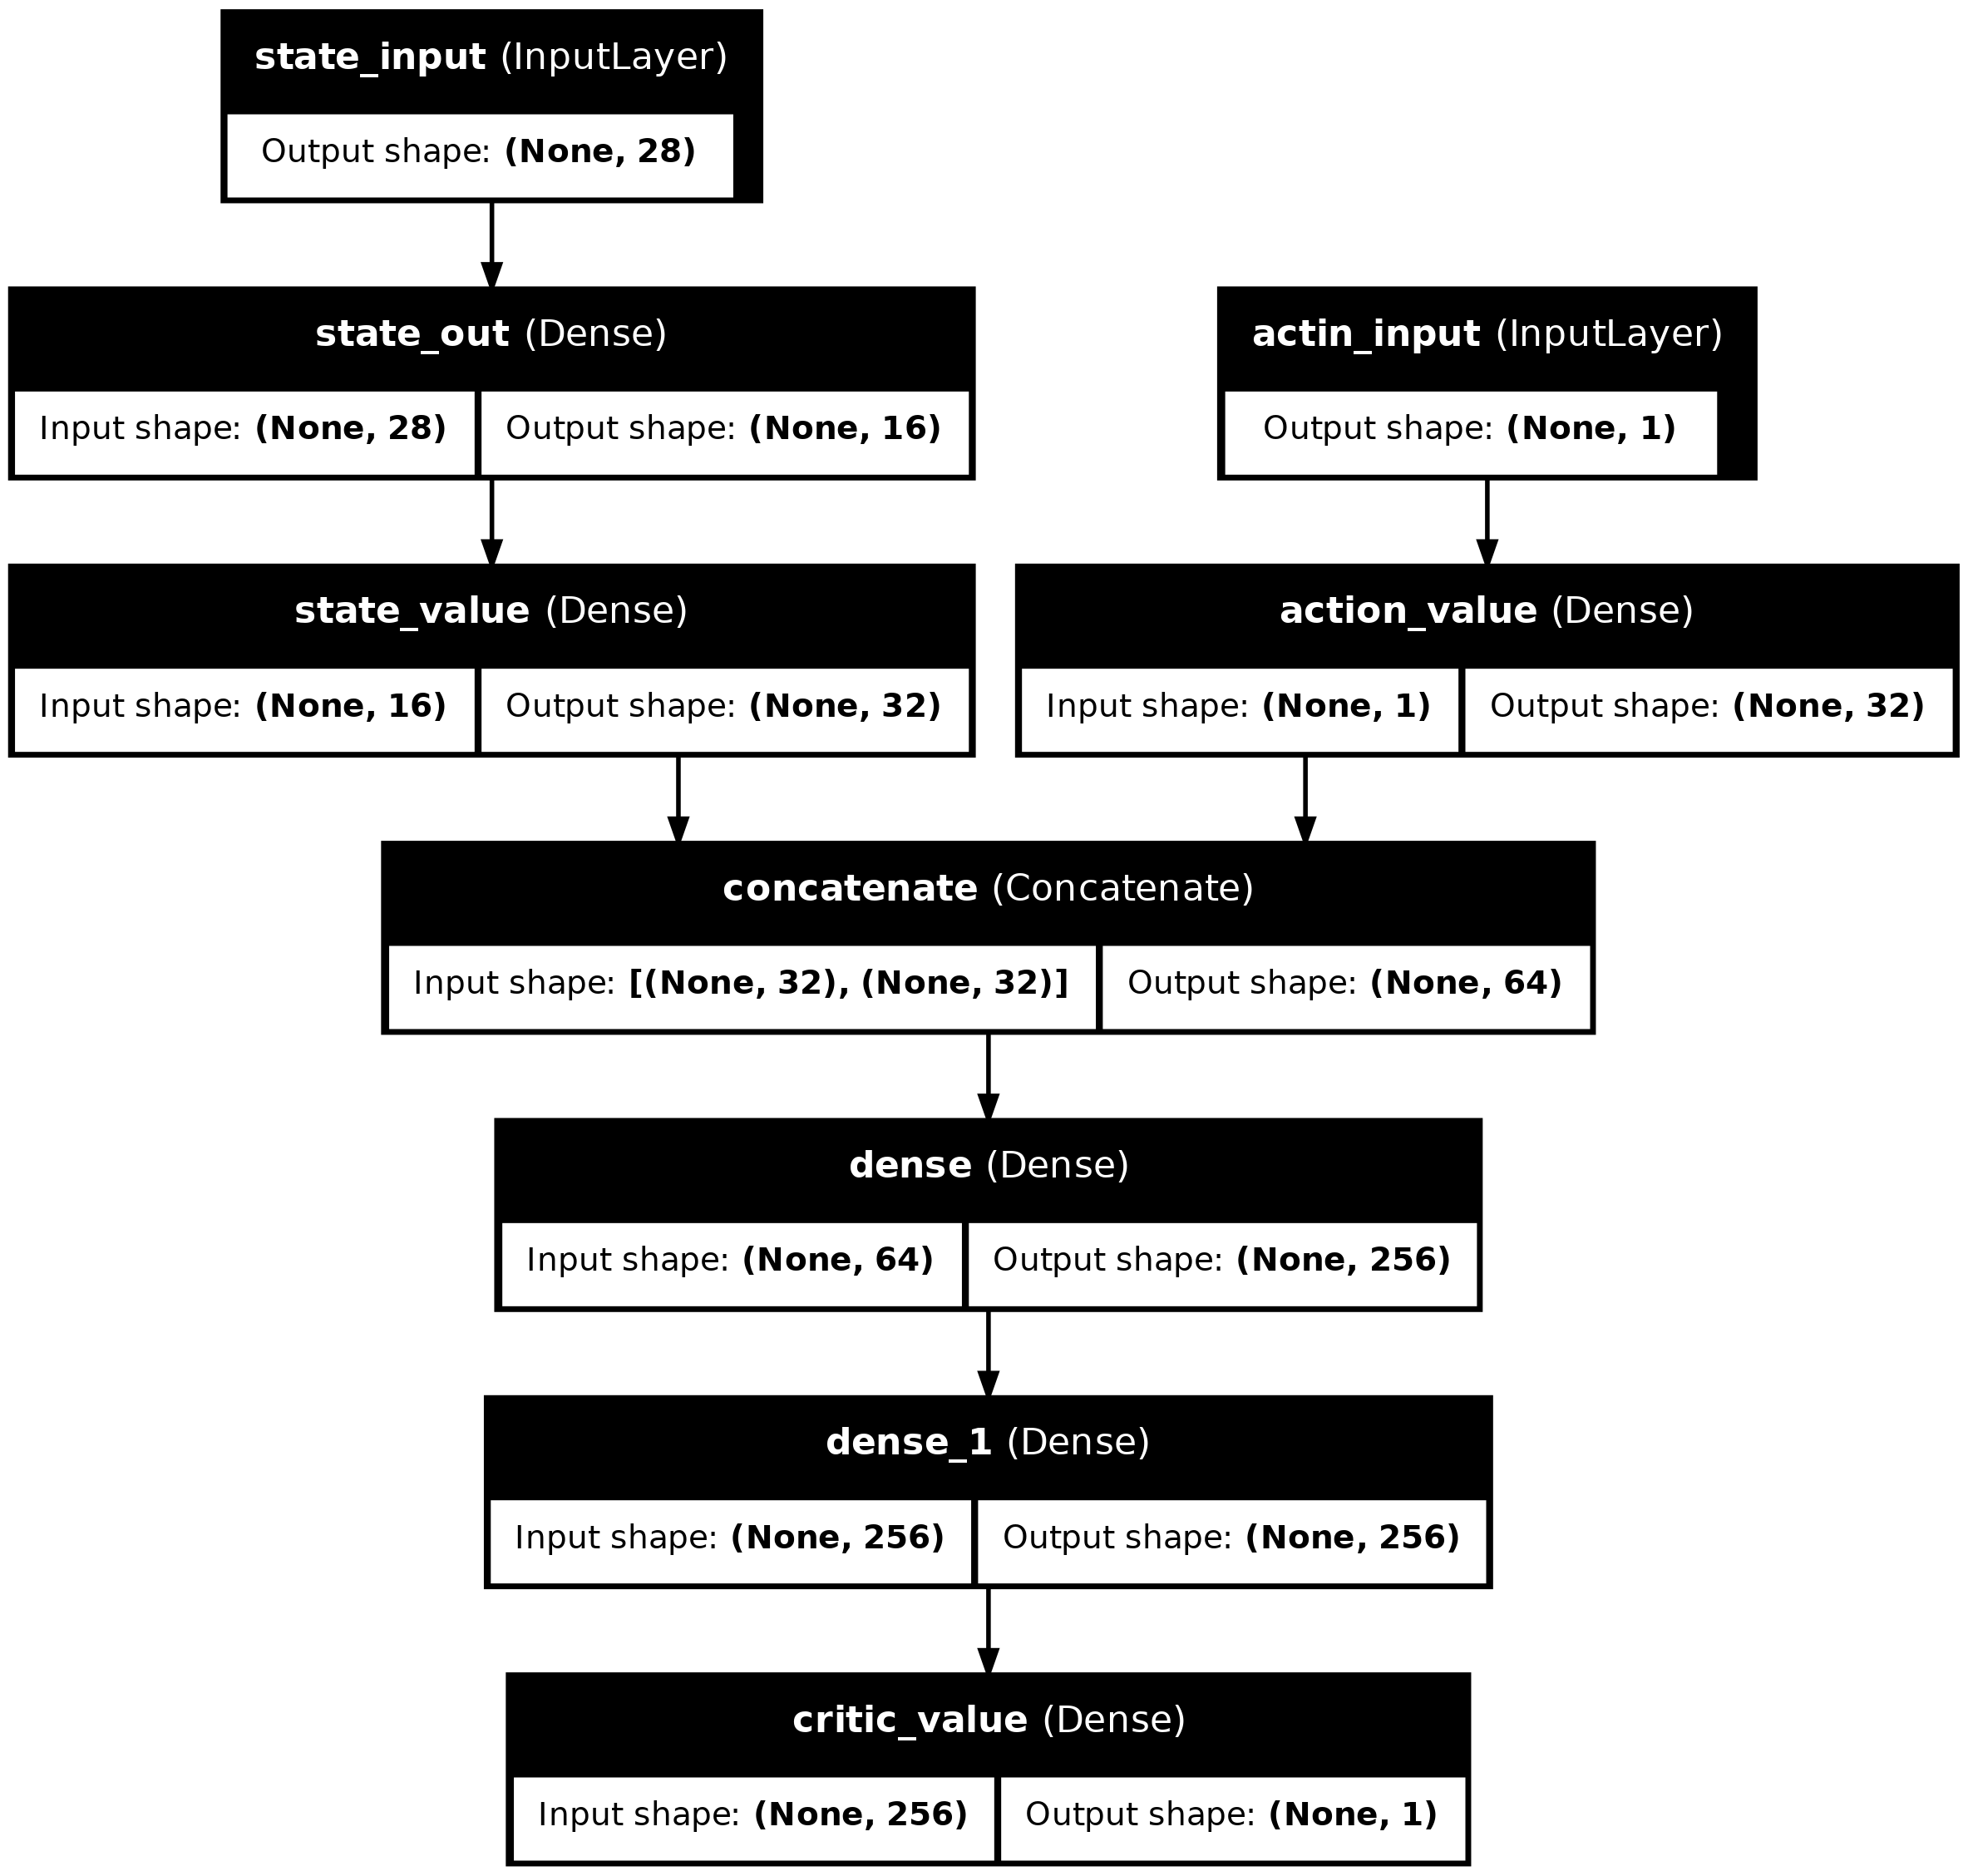
\includegraphics[width=0.6\textwidth]{./figures/critic_1_model.png}
    \caption{Critic network architecture.}
    \label{fig: critic network}
\end{figure}

The neural network that performs as actor/policy can be see in \ref{fig: actor network} and starts with an input layer, which consists of the state information. This layer is followed by a dense layer with 256 units, which processes the input data. The next layer, named "dense\_2," also contains 256 units and further refines the information. After these layers, the data moves to the output layer, called "output," which has a single unit. This unit generates the final output of the network, representing the action to be taken based on the input state. Additionally, there is a multiply layer named "multiply," which also has 1 unit. This layer helps scale the output appropriately.

\begin{figure}[ht]
    \centering
    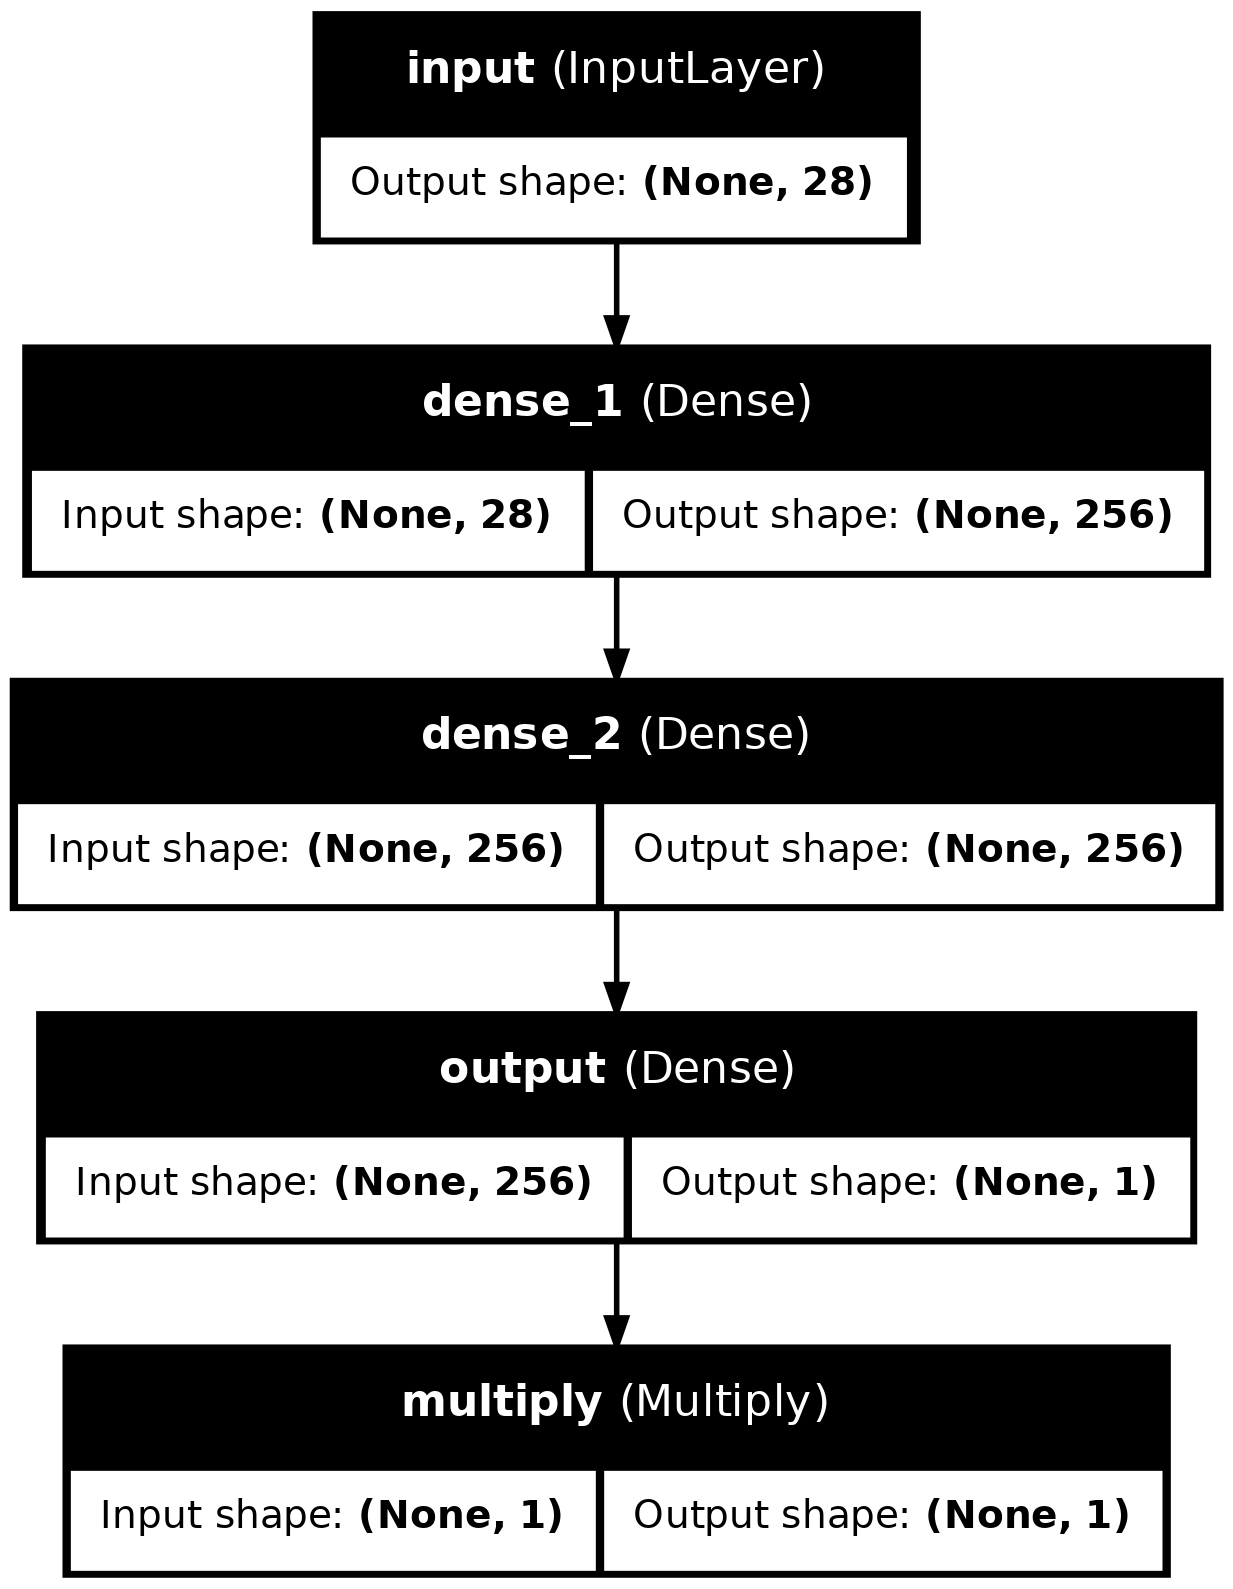
\includegraphics[width=0.4\textwidth]{./figures/actor_model.png}
    \caption{Actor network architecture.}
    \label{fig: actor network} 
\end{figure}

The input state of the network is the measurement received from the Lidar sensor which consist of 24 measurement of detected distances in angles around the mobile base plus the $x$ and $y$ distance of the goal from the mobile base.

The reward functions was designed to encourage the mobile base to get from its start point to the goal point in the less episodes possible and discouraging crash against any obstacle and keeping only on one side of the road. A crash of any kind is catastrophic for the episode. This function calculates a reward value that assists in guiding robot navigation by evaluating three primary factors: angular velocity, heading, and distance to the goal. The reward is designed to encourage efficient movement by balancing these elements.

The function takes several inputs:
\begin{itemize}
    \item \textbf{Heading angle}: Determines how well the robot's orientation aligns with the direction of the goal.
    \item \textbf{Angular velocity}: Measures the rate at which the robot adjusts its heading.
    \item \textbf{Start and current distance}: Helps assess whether the robot is moving closer to the goal.
    \item \textbf{Weight parameters}: Allow fine-tuning of the influence of angular velocity, heading, and distance improvement in the reward calculation.
\end{itemize}

By integrating these factors with adjustable weight parameters, the function produces a single reward value. This reward helps the robot make better navigation decisions by encouraging smooth directional adjustments, goal-focused movement, and minimizing unnecessary deviations.

To emulate the driving paradigm change, it was built an environment of a roundabout with line tracks emulated by walls as shown in figure \ref{fig: gazebo tb3 environment}. The blue layer represent what the robot "sees" through the Lidar scans. For each episode the robot is going to start from one side of the environment and should learn to go to the other side of the environment following only one track of the road, then, another agent is going to be trained with a brand new actor and critic models to follow the other track of the road so at the end there are two agents, one that knows how to traverse the environment following the right side and the other ones knows the other paradigm.

\begin{figure}[ht]
    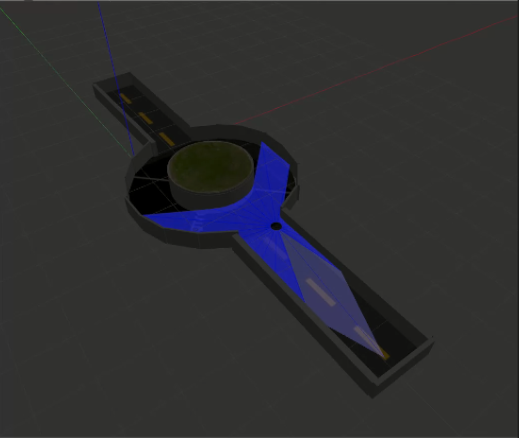
\includegraphics[width=0.7\textwidth]{./figures/experiment_environment_gazebo.png}
    \centering
    \caption{Turtlebot 3 in Gazebo simulator with roundabout environment.}
    \label{fig: gazebo tb3 environment}
\end{figure}

\hfil\break
Once the two agents are trained, The expert agents have to transfer the knowledge  to the new agents via transfer learning using equations \ref{eq: pre train gradient pi} and \ref{eq: pre train gradient Q} and measuring the transferred knowledge by 3 metrics given by the following equations:

\begin{equation}
    \begin{split}
        \text{Transfer ratio} & = \frac{\text{Ultimate performance with TL}}{\text{Ultimate performance with no TL}} \\
        Mastery               & = \text{Ultimate performance of the} agent.                                          \\
        Pedagogy              & = \text{How many less episodes the TL agent takes than a 0 trained agent.}
    \end{split}
\end{equation}

Where the $Ultimate performance$ means the return of the episode or the discounted cumulative reward achieved by the agent at the end of the episode.

\section{Experiments}
\subsection{Carla}
CARLA simulations were performed in the Town 5 environment shown in figure \ref{fig:town 5 carla}. The agent was trained to learn how to traverse the environment and achieve the most reward possible while maintaining a speed of $50km/h$. The only metric used to measure the performance of the agent was the reward function.

\subsection{Gazebo Roundabout}
The Gazebo simulations were divided into four parts:

\begin{enumerate}
    \item Training an agent to learn how to traverse the environment on the right side of the roundabout.
    \item Training an agent to learn how to traverse the environment on the left side of the roundabout. The reward function was slightly modified to include a penalty of $-1$ for each step the agent takes on the opposite side of the road.
    \item Training an expert agent that extends its learning to traverse the environment on the opposite side of the road.
    \item Training a transfer learning agent using the expert agent's critic and actor models.
\end{enumerate}

The metrics used to measure the performance of the agents were the average reward per episode, the number of steps taken, the average reward in the past 50 episode, the Q values for each network, the average loss value for each network and Q value difference.